% Options for packages loaded elsewhere
\PassOptionsToPackage{unicode}{hyperref}
\PassOptionsToPackage{hyphens}{url}
\documentclass[
]{article}
\usepackage{xcolor}
\usepackage[margin=1in]{geometry}
\usepackage{amsmath,amssymb}
\setcounter{secnumdepth}{5}
\usepackage{iftex}
\ifPDFTeX
  \usepackage[T1]{fontenc}
  \usepackage[utf8]{inputenc}
  \usepackage{textcomp} % provide euro and other symbols
\else % if luatex or xetex
  \usepackage{unicode-math} % this also loads fontspec
  \defaultfontfeatures{Scale=MatchLowercase}
  \defaultfontfeatures[\rmfamily]{Ligatures=TeX,Scale=1}
\fi
\usepackage{lmodern}
\ifPDFTeX\else
  % xetex/luatex font selection
\fi
% Use upquote if available, for straight quotes in verbatim environments
\IfFileExists{upquote.sty}{\usepackage{upquote}}{}
\IfFileExists{microtype.sty}{% use microtype if available
  \usepackage[]{microtype}
  \UseMicrotypeSet[protrusion]{basicmath} % disable protrusion for tt fonts
}{}
\makeatletter
\@ifundefined{KOMAClassName}{% if non-KOMA class
  \IfFileExists{parskip.sty}{%
    \usepackage{parskip}
  }{% else
    \setlength{\parindent}{0pt}
    \setlength{\parskip}{6pt plus 2pt minus 1pt}}
}{% if KOMA class
  \KOMAoptions{parskip=half}}
\makeatother
\usepackage{longtable,booktabs,array}
\newcounter{none} % for unnumbered tables
\usepackage{calc} % for calculating minipage widths
% Correct order of tables after \paragraph or \subparagraph
\usepackage{etoolbox}
\makeatletter
\patchcmd\longtable{\par}{\if@noskipsec\mbox{}\fi\par}{}{}
\makeatother
% Allow footnotes in longtable head/foot
\IfFileExists{footnotehyper.sty}{\usepackage{footnotehyper}}{\usepackage{footnote}}
\makesavenoteenv{longtable}
\usepackage{graphicx}
\makeatletter
\newsavebox\pandoc@box
\newcommand*\pandocbounded[1]{% scales image to fit in text height/width
  \sbox\pandoc@box{#1}%
  \Gscale@div\@tempa{\textheight}{\dimexpr\ht\pandoc@box+\dp\pandoc@box\relax}%
  \Gscale@div\@tempb{\linewidth}{\wd\pandoc@box}%
  \ifdim\@tempb\p@<\@tempa\p@\let\@tempa\@tempb\fi% select the smaller of both
  \ifdim\@tempa\p@<\p@\scalebox{\@tempa}{\usebox\pandoc@box}%
  \else\usebox{\pandoc@box}%
  \fi%
}
% Set default figure placement to htbp
\def\fps@figure{htbp}
\makeatother
% definitions for citeproc citations
\NewDocumentCommand\citeproctext{}{}
\NewDocumentCommand\citeproc{mm}{%
  \begingroup\def\citeproctext{#2}\cite{#1}\endgroup}
\makeatletter
 % allow citations to break across lines
 \let\@cite@ofmt\@firstofone
 % avoid brackets around text for \cite:
 \def\@biblabel#1{}
 \def\@cite#1#2{{#1\if@tempswa , #2\fi}}
\makeatother
\newlength{\cslhangindent}
\setlength{\cslhangindent}{1.5em}
\newlength{\csllabelwidth}
\setlength{\csllabelwidth}{3em}
\newenvironment{CSLReferences}[2] % #1 hanging-indent, #2 entry-spacing
 {\begin{list}{}{%
  \setlength{\itemindent}{0pt}
  \setlength{\leftmargin}{0pt}
  \setlength{\parsep}{0pt}
  % turn on hanging indent if param 1 is 1
  \ifodd #1
   \setlength{\leftmargin}{\cslhangindent}
   \setlength{\itemindent}{-1\cslhangindent}
  \fi
  % set entry spacing
  \setlength{\itemsep}{#2\baselineskip}}}
 {\end{list}}
\usepackage{calc}
\newcommand{\CSLBlock}[1]{\hfill\break\parbox[t]{\linewidth}{\strut\ignorespaces#1\strut}}
\newcommand{\CSLLeftMargin}[1]{\parbox[t]{\csllabelwidth}{\strut#1\strut}}
\newcommand{\CSLRightInline}[1]{\parbox[t]{\linewidth - \csllabelwidth}{\strut#1\strut}}
\newcommand{\CSLIndent}[1]{\hspace{\cslhangindent}#1}
\setlength{\emergencystretch}{3em} % prevent overfull lines
\providecommand{\tightlist}{%
  \setlength{\itemsep}{0pt}\setlength{\parskip}{0pt}}
\usepackage{amsmath, amssymb}
\usepackage{graphicx}
\usepackage{float}
\usepackage{placeins}
\usepackage{booktabs}
\usepackage{xcolor}
\usepackage{caption}
\captionsetup[table]{position=below,skip=6pt}
\usepackage{tikz}
\usetikzlibrary{arrows.meta,positioning,shadows,calc}
\usepackage{booktabs}
\usepackage{longtable}
\usepackage{array}
\usepackage{multirow}
\usepackage{wrapfig}
\usepackage{float}
\usepackage{colortbl}
\usepackage{pdflscape}
\usepackage{tabu}
\usepackage{threeparttable}
\usepackage{threeparttablex}
\usepackage[normalem]{ulem}
\usepackage{makecell}
\usepackage{xcolor}
\usepackage{bookmark}
\IfFileExists{xurl.sty}{\usepackage{xurl}}{} % add URL line breaks if available
\urlstyle{same}
\hypersetup{
  hidelinks,
  pdfcreator={LaTeX via pandoc}}

\author{}
\date{\vspace{-2.5em}}

\begin{document}

{
\setcounter{tocdepth}{2}
\tableofcontents
}
\begin{titlepage}
\begin{center}
    
\includegraphics[width=7cm]{./logo.jpg}
\vspace{0.5in}

    \LARGE{MSc Thesis for Health Data Science}

    \Huge{A Bayesian Time-Series Framework for Comparing On Trolley Counts Across Irish HSE Health Regions}

    \Large{Lucas Henry, Evan Bergin}

    \Large{Supervisors: Dr. Carl Scarrott, Dr. John Ferguson}

    \Large{XXXX 2026}

\end{center}
\end{titlepage}

\clearpage
\newpage

\underline{Declaration}

We hereby certify that this material, which we now submit for assessment on the programme of study leading to the award of Master of Science is entirely our own work and had not been taken from the work of others or Artificial Intelligence, save and to the extent that such work has been cited and acknowledged within the text of our work.

ID: 25252089

Date:

\newpage

\tableofcontents

\newpage

\section{\texorpdfstring{Introduction \label{chap:intro}}{Introduction }}\label{introduction}

\section{\texorpdfstring{Data \label{chap:data}}{Data }}\label{data}

The on trolley counts are sourced from the publicly available HSE Urgent and Emergency Report daily tables (Health Service Executive, 2026).
The data set was collected from January 1st 2023 to April 5th 2026.
Analysis used total on trolley counts.
During the scraping process, daily counts were aggregated into weekly counts.
Hospitals were aggregated into regions.

\subsection{\texorpdfstring{Scraping \label{sect:data-pipeline}}{Scraping }}\label{scraping}

A pipeline was created to extract daily on trolley counts from each HSE hospital and transform them into weekly counts for each region.
First by scraping the daily reports, which are published as HTML tables into a PostgreSQL database.
Daily on trolley counts are then aggregated into weekly counts by summing over each week, with Monday designated as the first day of the week.
Hospitals were aggregated into regions by summing their weekly counts into a weekly total counts per region.
Prior to model fit counts were scaled into rates. Scraping code can be found on Github (Henry \& Bergin, 2026).

\begin{figure}[h]
\centering
\resizebox{\textwidth}{!}{%
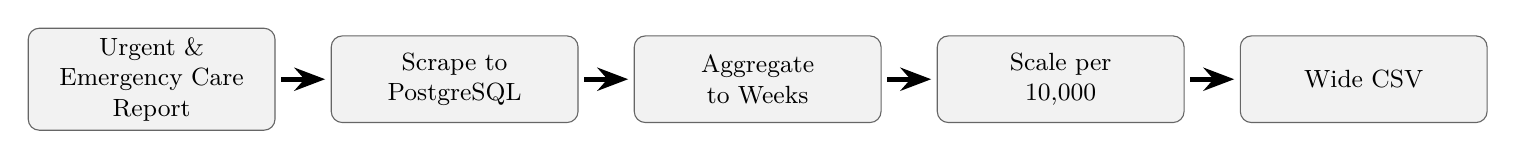
\begin{tikzpicture}[
  node distance=0.7cm,
  box/.style={
    rectangle, rounded corners=4pt,
    draw=black!60, fill=gray!10,
    text width=2.9cm, minimum height=1.1cm,
    align=center, font=\small
  },
  arr/.style={->, line width=1.8pt, >=Stealth, shorten >=2pt, shorten <=2pt}
]
  \node[box] (src)   {Urgent \&\\ Emergency Care\\ Report};
  \node[box, right=of src]   (db)    {Scrape to\\ PostgreSQL};
  \node[box, right=of db]    (agg)   {Aggregate\\ to Weeks};
  \node[box, right=of agg]   (scale) {Scale per\\ 10{,}000};
  \node[box, right=of scale] (csv)   {Wide CSV};

  \draw[arr] (src)   -- (db);
  \draw[arr] (db)    -- (agg);
  \draw[arr] (agg)   -- (scale);
  \draw[arr] (scale) -- (csv);
\end{tikzpicture}%
}% end resizebox
\caption{Data pipeline from source to model input.}
\label{fig:data-pipeline}
\end{figure}

\subsection{\texorpdfstring{Exploratory Data Analysis \label{sect:data-EDA}}{Exploratory Data Analysis }}\label{exploratory-data-analysis}

Figure \ref{fig:eda-weekly-overview} shows the weekly on trolley counts for each region from the start of 2023, to April 2026.
Sharp dips in patients on trolleys occur just prior to each new year, observed close up in figure \ref{fig:eda-events}A.
This can be explained by the HSE's annual practice of discharging patients during christmas time to prepare for the January surge {[}Department of Health (2023){]}.
\FloatBarrier
\pandocbounded{\includegraphics[keepaspectratio,alt={\label{fig:eda-weekly-overview}Weekly total on-trolley counts by HSE region from 2023 to 2026. Light blue bands mark the New Year weeks across all regions; the light red band marks the Mid West reset window (8--19 August 2024).}]{ThesisDraft_v2_files/figure-latex/eda-weekly-overview-1.pdf}}

\FloatBarrier

The sharp dip see in the Mid West is explained by HSE Mid West's action in delaying scheduled care to focus on unscheduled care @{[}{]}.
The delay is visualised in the red shaded region in figure \ref{fig:eda-events}B.
During this time, total patients on trolleys are reduced to near 0, before rebounding.

\begin{figure}
\centering
\pandocbounded{\includegraphics[keepaspectratio,alt={\label{fig:eda-events}Top: New Year close-up for HSE Dublin and Midlands, weekly total trolleys in the 8 weeks either side of 1 January for each year in the series. Bottom: HSE Mid West weekly trolley totals from May to November 2024; the shaded window marks the 8--19 August reset period, during which inpatient, outpatient and day cases were deferred.}]{ThesisDraft_v2_files/figure-latex/eda-events-1.pdf}}
\caption{\label{fig:eda-events}Top: New Year close-up for HSE Dublin and Midlands, weekly total trolleys in the 8 weeks either side of 1 January for each year in the series. Bottom: HSE Mid West weekly trolley totals from May to November 2024; the shaded window marks the 8--19 August reset period, during which inpatient, outpatient and day cases were deferred.}
\end{figure}

\begin{figure}
\centering
\pandocbounded{\includegraphics[keepaspectratio,alt={\label{fig:eda-psd}Smoothed periodogram (Daniell windowed) of weekly trolley counts for each HSE region. The dashed line marks the 52-week period.}]{ThesisDraft_v2_files/figure-latex/eda-psd-1.pdf}}
\caption{\label{fig:eda-psd}Smoothed periodogram (Daniell windowed) of weekly trolley counts for each HSE region. The dashed line marks the 52-week period.}
\end{figure}

\begin{figure}
\centering
\pandocbounded{\includegraphics[keepaspectratio,alt={\label{fig:eda-pacf}Partial autocorrelation function of weekly trolley totals for HSE Dublin and Midlands. The lag-1 bar is large and well outside the 95\% confidence band, while higher lags fall within it.}]{ThesisDraft_v2_files/figure-latex/eda-pacf-1.pdf}}
\caption{\label{fig:eda-pacf}Partial autocorrelation function of weekly trolley totals for HSE Dublin and Midlands. The lag-1 bar is large and well outside the 95\% confidence band, while higher lags fall within it.}
\end{figure}

\begin{figure}
\centering
\pandocbounded{\includegraphics[keepaspectratio,alt={\label{fig:eda-region-pop}2022 Health Region population.}]{ThesisDraft_v2_files/figure-latex/eda-region-pop-1.pdf}}
\caption{\label{fig:eda-region-pop}2022 Health Region population.}
\end{figure}

\FloatBarrier

\section{\texorpdfstring{Methods \label{chap:methods}}{Methods }}\label{methods}

The on trolley counts are scaled to three different rates to understand their impact on ranks between regions. Informed by EDA, the models were specified.

\subsection{\texorpdfstring{Response Scaling \label{sect:standardisation}}{Response Scaling }}\label{response-scaling}

\subsubsection{Population scaling}\label{population-scaling}

The on trolley counts were standardised to a rate of count per 10,000 people in each health region to control for catchment population size:

\[
y_{i,t} = \frac{\text{weekly trolley count}_{i,t}}{\text{health region catchment population}_i} \times 10{,}000.
\]

\subsubsection{Budget scaling}\label{budget-scaling}

Weekly trolley counts scaled by the 2026 HSE regional budget allocation, expressing the outcome as trolleys per billions of euros allocated to the region:

\[
y_{i,t} = \frac{\text{weekly trolley count}_{i,t}}{\text{health region budget in billion (€)}_i}.
\]

This controls for funding differentials: a region receiving a larger allocation is expected to handle a proportionally larger patient volume.

\subsubsection{Bed scaling}\label{bed-scaling}

Weekly trolley counts scaled by the number of inpatient beds in each region as of June 2025 inquiry:

\[
y_{i,t} = \frac{\text{weekly trolley count}_{i,t}}{\text{number of health region inpatient beds}_i} \times 100.
\]

This controls for space capacity differentials: a region allocated more space is expected to handle a larger patient volume.

\subsection{\texorpdfstring{Model Development \label{sect:model-development}}{Model Development }}\label{model-development}

Models were developed iteratively with increasing complexity as described in Gelman (2004). Model iteration can be visualised in appendix figure \ref{fig:model-inheritance}. Components were added to the model according to the residual patterns, resulting in the base model \eqref{eq:base-likelihood}.

The base model likelihood initialises at \(t=1\) and propagates an AR(1) carryover at \(t>1\).

\begin{equation}
y_{i,1} \sim \mathcal{N}(\mu_{i,1},\ \tau_i^{-1})
\label{eq:base-likelihood-init}
\end{equation}

\begin{equation}
y_{i,t} \sim \mathcal{N}\!\left(\mu_{i,t} + \mathcal{E}^{1}_{i,t},\ \tau_i^{-1}\right), \quad t > 1
\label{eq:base-likelihood}
\end{equation}

The AR(1) term captures week-to-week autocorrelation in the residuals.

\begin{equation}
\mathcal{E}^{1}_{i,t} = \phi\,(y_{i,t-1} - \mu_{i,t-1})
\label{eq:base-ar1}
\end{equation}

The mean function decomposes the expected trolley rate into a baseline level (\(\alpha_i\)), an annual cycle (\(\mathcal{C}_{i,t}^{52}\)), a regional New Year effect (\(\mathcal{R}_{i,t}\)), and a Mid West funding reset (\(\mathcal{W}_{i,t}\)).

\begin{equation}
\mu_{i,t} = \alpha_i + \mathcal{C}_{i,t}^{52} + \mathcal{R}_{i,t} + \mathcal{W}_{i,t}
\label{eq:base-mean}
\end{equation}

The annual cycle is captured with the \(\mathcal{C}_{i,t}^{52}\) component.

\begin{equation}
\mathcal{C}_{i,t}^{52} = \beta_i \cos\!\left(\tfrac{2\pi t}{52}\right) + \gamma_i \sin\!\left(\tfrac{2\pi t}{52}\right)
\end{equation}

The regional New Year effect allows each region to respond differently across the three week New Year window.

\begin{equation}
\begin{aligned}
\mathcal{R}_{i,t} &= \delta_{\text{pre},i}\,\mathbf{1}(t \bmod 52 = 0) \\
                  &+ \delta_{\text{mid},i}\,\mathbf{1}(t \bmod 52 = 1) \\
                  &+ \delta_{\text{post},i}\,\mathbf{1}(t \bmod 52 = 2)
\end{aligned}
\label{eq:base-newyear}
\end{equation}

In the Mid West region, from August 8th 2024 to August 19th 2024, cases deferred to focus on unscheduled care.
This is captured with the \(\mathcal{W}_{i,t}\) component:

\begin{equation}
\begin{aligned}
\mathcal{W}_{i,t} = \mathbf{1}(i = \text{HSE Mid West})\cdot\bigl(&\psi_{\text{pre}}\,\mathbf{1}(t = 86) \\
  +\,&\psi_{\text{mid}}\,\mathbf{1}(t = 87) \\
  +\,&\psi_{\text{post}}\,\mathbf{1}(t = 88)\bigr)
\end{aligned}
\label{eq:base-mwreset}
\end{equation}

Extending the base model described above, two models were added. One with an added AR(2) component.

\begin{equation}
  \begin{aligned}
    &y_{i,t} \sim \mathcal{N}\!\left(\mu_{i,t} + 
    \mathcal{E}^{1}_{i,t} + 
    \mathcal{E}^{2}_{i,t},\ \tau_i^{-1}\right)\\
    &\mu_{i,t} = \alpha_i + \mathcal{C}_{i,t}^{52} + \mathcal{R}_{i,t} + \mathcal{W}_{i,t}
  \end{aligned}
  \label{eq:extended-AR2}
\end{equation}

A second with an added 6-month cycle.

\begin{equation}
  \begin{aligned}
    &y_{i,t} \sim \mathcal{N}\!\left(\mu_{i,t} + 
    \mathcal{E}^{1}_{i,t},\ \tau_i^{-1}\right)\\
    &\mu_{i,t} = \alpha_i + 
    \mathcal{C}_{i,t}^{52} + 
    \mathcal{C}_{i,t}^{26} + \mathcal{R}_{i,t} + \mathcal{W}_{i,t}
  \end{aligned}
  \label{eq:extended-6-month}
\end{equation}

\subsection{\texorpdfstring{Posterior Sampling and Bayesian Ranking \label{sect:ranking}}{Posterior Sampling and Bayesian Ranking }}\label{posterior-sampling-and-bayesian-ranking}

Posterior sampling was preformed using \emph{Just another Gibbs sampler} (\emph{JAGs})(Plummer, 2003), implemented by pyJAGS (Nowotny, 2024), a Python interface to JAGS. Health region baselines, \(\alpha^s_j\), were used for ranking. Where \(j\) is one of the 6 HSE health regions, \(j\in\{1,...,6\}\), and \(s\) is the draw index, for \(s\in\{1,...,n\}\) and total samples is defined as \(n=20{,}000\).
\[
  A =
  \left[ {\begin{array}{ccccc}
    \alpha_1^1 & \cdots & \alpha_j^1 & \cdots & \alpha_6^1\\
    \vdots  &        & \vdots\\
    \alpha_1^s & \cdots & \alpha_j^s& \cdots & \alpha_6^s\\
    \vdots  &        & \vdots\\
    \alpha_1^n & \cdots & \alpha_j^n & \cdots & \alpha_6^n\\
  \end{array} } \right]
\]
Ranks follow the posterior ranking approach of Laird \& Louis (1989). Where each sample is posterior sample is ranked to form rank distribution, \(R\).
\[
  R =
  \left[ {\begin{array}{ccccc}
    r_1^1 & \cdots & r_j^1 & \cdots & r_6^1\\
    \vdots  &        & \vdots\\
    r_1^s & \cdots & r_j^s& \cdots & r_6^s\\
    \vdots  &        & \vdots\\
    r_1^n & \cdots & r_j^n & \cdots & r_6^n\\
  \end{array} } \right]
\]
Where \(r_j^s=\text{rank}(\alpha_j^s)=\sum^6_{i=1}I(\alpha_j^s>\alpha_i^s)\). Given a tie, ranks were increased by \(\frac{1}{2}\) steps for each tied value:
\[r^s_j= \sum_{i=1}^{6} \left[ \mathbf{1}(\alpha_j^s > \alpha_i^s) + \tfrac{1}{2}\mathbf{1}(\alpha_j^s = \alpha_i^s) \right]\]
Then posterior rank averages, \(\hat{r}_i\), were calculated taking the mean across samples.
\[\hat{r}_j=\displaystyle \frac{1}{n}\sum^n_{s=1} r_j^s\]
\[
  \hat{R} =
  \left[ {\begin{array}{ccccc}
    \hat{r}_1, \hat{r}_2, \hat{r}_3, \hat{r}_4, \hat{r}_5,  \hat{r}_6
  \end{array} } \right]
\]
Then posterior ranked averages were ranked once again to achieve ranked posterior ranked averages were calculated.
\[
r_j^*=rank(\alpha_j^*)=\sum^6_{i=1}I(\alpha_j^*>\alpha_i^*)
\]
\[
  R^* =
  \left[ {\begin{array}{ccccc}
    r^*_1, r^*_2, r^*_3, r^*_4, r^*_5, r^*_6
  \end{array} } \right]
\]
Where \(r_j^*=rank(\hat{r}_j)=\sum^6_{i=1}I(\hat{r}_j>\hat{r}_i)\).

\subsection{\texorpdfstring{Code and Data Availability \label{sect:code}}{Code and Data Availability }}\label{code-and-data-availability}

\textit{[Placeholder: link to GitHub repository, languages and tools used (Python, R, JAGS), and note that source data is publicly available from the HSE Urgent and Emergency Care portal.]}

\section{\texorpdfstring{Results \label{chap:results}}{Results }}\label{results}

\subsection{\texorpdfstring{Model Comparison \label{sect:dic-results}}{Model Comparison }}\label{model-comparison}

\subsubsection{Regional Baseline}\label{regional-baseline}

\subsubsection{Week-to-Week Autocorrelation}\label{week-to-week-autocorrelation}

\subsubsection{Annual Cycle}\label{annual-cycle}

\subsubsection{Regional Rankings}\label{regional-rankings}

\newpage

\section{\texorpdfstring{Discussion \label{chap:Discussion}}{Discussion }}\label{discussion}

\newpage

\section{References}\label{references}

\protect\phantomsection\label{refs}
\begin{CSLReferences}{1}{0}
\bibitem[\citeproctext]{ref-department_of_health_minister_2023}
Department of Health. (2023). Minister for {Health} thanks healthcare workers for delivering 20\% reduction in trolley numbers in last 6 months of 2023. In \emph{Gov.ie}. \url{https://www.gov.ie/en/department-of-health/press-releases/minister-for-health-thanks-healthcare-workers-for-delivering-20-reduction-in-trolley-numbers-in-last-6-months-of-2023/}

\bibitem[\citeproctext]{ref-gelman_exploratory_2004}
Gelman, A. (2004). Exploratory {Data} {Analysis} for {Complex} {Models}. \emph{Journal of Computational and Graphical Statistics}, \emph{13}(4), 755--779. \url{https://doi.org/10.1198/106186004X11435}

\bibitem[\citeproctext]{ref-HSE2026}
Health Service Executive. (2026). \emph{Urgent and emergency care report}. \url{https://www2.hse.ie/services/urgent-emergency-care-report/}

\bibitem[\citeproctext]{ref-henry_hse_2026}
Henry, L., \& Bergin, E. (2026). \emph{{HSE} {Urgent} {Care} {Report} {Bayesian} {Analysis}}. \url{https://github.com/hotsoupisgood/scraping-hse-trolly-data}

\bibitem[\citeproctext]{ref-Laird1989}
Laird, N. M., \& Louis, T. A. (1989). Empirical {B}ayes ranking methods. \emph{Journal of Educational Statistics}, \emph{14}(1), 29--46. \url{https://doi.org/10.3102/10769986014001029}

\bibitem[\citeproctext]{ref-Nowotny2024pyjags}
Nowotny, M. (2024). \emph{{pyJAGS}: A {P}ython interface to {JAGS}} (Version 2.4.0) {[}Computer software{]}. \url{https://github.com/michaelnowotny/pyjags}

\bibitem[\citeproctext]{ref-Plummer2003}
Plummer, M. (2003). {JAGS}: A program for analysis of {B}ayesian graphical models using {G}ibbs sampling. \emph{Proceedings of the 3rd International Workshop on Distributed Statistical Computing ({DSC} 2003)}. \url{https://www.r-project.org/conferences/DSC-2003/Proceedings/Plummer.pdf}

\end{CSLReferences}

\newpage

\section{Appendix}\label{appendix}

\subsection{Model Inheritance}\label{model-inheritance}

\definecolor{boxblue}{HTML}{e8f4f8}
\definecolor{boxborder}{HTML}{2c3e50}
\definecolor{boxgrey}{HTML}{f0f0f0}
\definecolor{bordergrey}{HTML}{999999}
\definecolor{divider}{HTML}{aaaaaa}

\tikzset{
  model/.style={
    rectangle, rounded corners=4pt,
    draw=boxborder, fill=boxblue,
    minimum width=3.2cm, minimum height=1.1cm,
    text width=3.0cm, align=center, font=\small,
    drop shadow={shadow xshift=0.5mm, shadow yshift=-0.5mm}
  },
  unselected/.style={
    rectangle, rounded corners=4pt,
    draw=boxborder, fill=boxgrey,
    minimum width=3.2cm, minimum height=1.1cm,
    text width=3.0cm, align=center, font=\small,
    drop shadow={shadow xshift=0.5mm, shadow yshift=-0.5mm}
  },
  row label/.style={
    font=\scriptsize\itshape, text=bordergrey,
    align=right, text width=2.2cm
  },
  arr/.style={-Stealth, thick, color=boxborder},
  arr branch/.style={-Stealth, thin, color=boxborder}
}

\begin{figure}[h]
\centering
\resizebox{\textwidth}{!}{%
\begin{tikzpicture}[node distance=1.8cm and 0.3cm]

  % --- Row 0: AR baseline ---
  \node[model] (v0_1) {\textbf{v0.1}\\AR(1) Only};

  % --- Row 1: Cycle ---
  \node[model, below=of v0_1] (v1_1) {\textbf{v1.1}\\Annual Cycle};

  % --- Row 2: Event + MW reset ---
  \node[model, below=of v1_1] (v2_1) {\textbf{v2.1}\\Regional NY + MW Reset};
  \node[unselected, left=of v2_1] (v2_3) {\textbf{v2.3}\\Regional New Year};
  \node[unselected, left=of v2_3] (v2_2) {\textbf{v2.2}\\Global New Year};
  \node[unselected, right=of v2_1] (v2_4) {\textbf{v2.4}\\MW Reset Only};

  % --- Row 3: Extensions (unselected robustness checks) ---
  \node[unselected, below=of v2_1] (v3_2) {\textbf{v3.2}\\v2.1 + 6-Month Cycle};
  \node[unselected, left=of v3_2] (v3_1) {\textbf{v3.1}\\v2.1 + 2-Month Cycle};
  \node[unselected, right=of v3_2] (v3_3) {\textbf{v3.3}\\v2.1 + AR(2)};

  % --- Row side labels ---
  \coordinate (llabel) at ($(v2_2.west) + (-0.4, 0)$);
  \node[row label, anchor=east] at (llabel |- v0_1) {AR order};
  \node[row label, anchor=east] at (llabel |- v1_1) {Cycle type};
  \node[row label, anchor=east] at (llabel |- v2_1) {Event + MW reset};
  \node[row label, anchor=east] at (llabel |- v3_2) {Extensions};

  % --- Horizontal dividers ---
  \coordinate (left)  at ($(v2_2.west) + (-2.8, 0)$);
  \coordinate (right) at ($(v2_4.east)  + ( 0.4, 0)$);

  \draw[dashed, color=divider, line width=0.6pt]
    ($(left |- v0_1.south) + (0,-0.5)$) -- ($(right |- v0_1.south) + (0,-0.5)$);
  \draw[dashed, color=divider, line width=0.6pt]
    ($(left |- v1_1.south) + (0,-0.5)$) -- ($(right |- v1_1.south) + (0,-0.5)$);
  \draw[dashed, color=divider, line width=0.6pt]
    ($(left |- v2_1.south) + (0,-0.5)$) -- ($(right |- v2_1.south) + (0,-0.5)$);

  % --- Diagram title ---
  \node[font=\small\itshape, text=bordergrey,
    above=0.7cm of v0_1, xshift=0cm, anchor=center]
    {Population-scaled response: trolleys per 10{,}000 population per week};

  % --- Spine arrows ---
  \draw[arr] (v0_1) -- (v1_1);
  \draw[arr] (v1_1) -- (v2_1);

\end{tikzpicture}%
}% end resizebox
\caption{Model inheritance diagram. Spine nodes (blue) form the selected
model sequence; grey nodes were tested variants. Thick arrows indicate the
selected path; thin arrows indicate branches.}
\label{fig:model-inheritance}
\end{figure}

\subsection{Full Model Specifications}\label{full-model-specs}

\subsubsection*{Model v0.1}\label{model-v0.1}
\addcontentsline{toc}{subsubsection}{Model v0.1}

\begin{itemize}
\tightlist
\item
  AR(1) baseline; no cycle, no event effects
\end{itemize}

\textbf{Likelihood}

\[
\begin{aligned}
y_{i,1} &\sim \mathcal{N}(\mu_{i,1},\ \tau_i^{-1}) \\[4pt]
y_{i,t} &\sim \mathcal{N}\!\left(\mu_{i,t} + \mathcal{E}^{1}_{i,t},\ \tau_i^{-1}\right), \quad t > 1\\
\end{aligned}
\]
Where \(\mu_{i,t}\) is the baseline mean for region \(i\) at time \(t\).
\[
\begin{aligned}
\mu_{i,t} &= \alpha_i \\[4pt]
\end{aligned}
\]
\(\mathcal{E}^{1}_{i,t}\) is the AR(1) error term.
\[
\begin{aligned}
\mathcal{E}^{1}_{i,t} &= \phi\,(y_{i,t-1} - \mu_{i,t-1})\\
\end{aligned}
\]

\textbf{Priors}

\[
\begin{aligned}
\alpha_i &\sim \mathcal{N}(0,\ 0.001) \\[4pt]
\tau_i   &\sim \Gamma(0.001,\ 0.001) \\[4pt]
\phi     &\sim \mathrm{Uniform}(-1,\ 1)
\end{aligned}
\]

\subsubsection*{Model v1.1}\label{model-v1.1}
\addcontentsline{toc}{subsubsection}{Model v1.1}

\begin{itemize}
\tightlist
\item
  Extends v0.1; adds annual cycle
\end{itemize}

\textbf{Likelihood}

\[
\begin{aligned}
\mu_{i,t} &= \alpha_i
              + \beta_i \cos\!\left(\tfrac{2\pi t}{52}\right)
              + \gamma_i \sin\!\left(\tfrac{2\pi t}{52}\right) \\[4pt]
y_{i,1} &\sim \mathcal{N}(\mu_{i,1},\ \tau_i^{-1}) \\[4pt]
y_{i,t} &\sim \mathcal{N}\!\left(\mu_{i,t} + \phi\,(y_{i,t-1} - \mu_{i,t-1}),\ \tau_i^{-1}\right), \quad t > 1
\end{aligned}
\]

\textbf{Priors}

\[
\begin{aligned}
\alpha_i,\ \beta_i,\ \gamma_i &\sim \mathcal{N}(0,\ 0.001) \\[4pt]
\tau_i &\sim \Gamma(0.001,\ 0.001) \\[4pt]
\phi   &\sim \mathrm{Uniform}(-1,\ 1)
\end{aligned}
\]

\subsubsection*{\texorpdfstring{Model v2.1 \label{sect:model}}{Model v2.1 }}\label{model-v2.1}
\addcontentsline{toc}{subsubsection}{Model v2.1 \label{sect:model}}

\begin{itemize}
\tightlist
\item
  Extends v1.1; adds regional New Year effect and Mid West funding reset
\end{itemize}

\textbf{Likelihood}

\[
\begin{aligned}
\mu_{i,t} &= \alpha_i
              + \beta_i \cos\!\left(\tfrac{2\pi t}{52}\right)
              + \gamma_i \sin\!\left(\tfrac{2\pi t}{52}\right) \\[4pt]
           &\quad + \delta_{\text{pre},i}\,\mathbf{1}(t \bmod 52 = 0)
              + \delta_{\text{mid},i}\,\mathbf{1}(t \bmod 52 = 1)
              + \delta_{\text{post},i}\,\mathbf{1}(t \bmod 52 = 2) \\[4pt]
           &\quad + \bigl(\psi_{\text{pre}}\,\mathbf{1}(t = 86)
              + \psi_{\text{mid}}\,\mathbf{1}(t = 87)
              + \psi_{\text{post}}\,\mathbf{1}(t = 88)\bigr)\cdot\mathrm{mw}_i \\[4pt]
y_{i,1} &\sim \mathcal{N}(\mu_{i,1},\ \tau_i^{-1}) \\[4pt]
y_{i,t} &\sim \mathcal{N}\!\left(\mu_{i,t} + \phi\,(y_{i,t-1} - \mu_{i,t-1}),\ \tau_i^{-1}\right), \quad t > 1
\end{aligned}
\]

\textbf{Priors}

\[
\begin{aligned}
\alpha_i,\ \beta_i,\ \gamma_i &\sim \mathcal{N}(0,\ 0.001) \\[4pt]
\delta_{\text{pre},i},\ \delta_{\text{mid},i},\ \delta_{\text{post},i} &\sim \mathcal{N}(0,\ 0.001) \\[4pt]
\psi_{\text{pre}},\ \psi_{\text{mid}},\ \psi_{\text{post}} &\sim \mathcal{N}(0,\ 0.001) \\[4pt]
\tau_i &\sim \Gamma(0.001,\ 0.001) \\[4pt]
\phi   &\sim \mathrm{Uniform}(-1,\ 1)
\end{aligned}
\]

\subsubsection*{Model v2.2}\label{model-v2.2}
\addcontentsline{toc}{subsubsection}{Model v2.2}

\begin{itemize}
\tightlist
\item
  Extends v1.1; adds global New Year effect (shared across regions)
\end{itemize}

\textbf{Likelihood}

\[
\begin{aligned}
\mu_{i,t} &= \alpha_i
              + \beta_i \cos\!\left(\tfrac{2\pi t}{52}\right)
              + \gamma_i \sin\!\left(\tfrac{2\pi t}{52}\right) \\[4pt]
           &\quad + \delta_{\text{pre}}\,\mathbf{1}(t \bmod 52 = 0)
              + \delta_{\text{mid}}\,\mathbf{1}(t \bmod 52 = 1)
              + \delta_{\text{post}}\,\mathbf{1}(t \bmod 52 = 2) \\[4pt]
y_{i,1} &\sim \mathcal{N}(\mu_{i,1},\ \tau_i^{-1}) \\[4pt]
y_{i,t} &\sim \mathcal{N}\!\left(\mu_{i,t} + \phi\,(y_{i,t-1} - \mu_{i,t-1}),\ \tau_i^{-1}\right), \quad t > 1
\end{aligned}
\]

\textbf{Priors}

\[
\begin{aligned}
\alpha_i,\ \beta_i,\ \gamma_i &\sim \mathcal{N}(0,\ 0.001) \\[4pt]
\delta_{\text{pre}},\ \delta_{\text{mid}},\ \delta_{\text{post}} &\sim \mathcal{N}(0,\ 0.001) \\[4pt]
\tau_i &\sim \Gamma(0.001,\ 0.001) \\[4pt]
\phi   &\sim \mathrm{Uniform}(-1,\ 1)
\end{aligned}
\]

\subsubsection*{Model v2.3}\label{model-v2.3}
\addcontentsline{toc}{subsubsection}{Model v2.3}

\begin{itemize}
\tightlist
\item
  Extends v1.1; adds regional New Year effect (no MW reset)
\end{itemize}

\textbf{Likelihood}

\[
\begin{aligned}
\mu_{i,t} &= \alpha_i
              + \beta_i \cos\!\left(\tfrac{2\pi t}{52}\right)
              + \gamma_i \sin\!\left(\tfrac{2\pi t}{52}\right) \\[4pt]
           &\quad + \delta_{\text{pre},i}\,\mathbf{1}(t \bmod 52 = 0)
              + \delta_{\text{mid},i}\,\mathbf{1}(t \bmod 52 = 1)
              + \delta_{\text{post},i}\,\mathbf{1}(t \bmod 52 = 2) \\[4pt]
y_{i,1} &\sim \mathcal{N}(\mu_{i,1},\ \tau_i^{-1}) \\[4pt]
y_{i,t} &\sim \mathcal{N}\!\left(\mu_{i,t} + \phi\,(y_{i,t-1} - \mu_{i,t-1}),\ \tau_i^{-1}\right), \quad t > 1
\end{aligned}
\]

\textbf{Priors}

\[
\begin{aligned}
\alpha_i,\ \beta_i,\ \gamma_i &\sim \mathcal{N}(0,\ 0.001) \\[4pt]
\delta_{\text{pre},i},\ \delta_{\text{mid},i},\ \delta_{\text{post},i} &\sim \mathcal{N}(0,\ 0.001) \\[4pt]
\tau_i &\sim \Gamma(0.001,\ 0.001) \\[4pt]
\phi   &\sim \mathrm{Uniform}(-1,\ 1)
\end{aligned}
\]

\subsubsection*{Model v2.4}\label{model-v2.4}
\addcontentsline{toc}{subsubsection}{Model v2.4}

\begin{itemize}
\tightlist
\item
  Extends v1.1; adds Mid West funding reset (no New Year effect)
\end{itemize}

\textbf{Likelihood}

\[
\begin{aligned}
\mu_{i,t} &= \alpha_i
              + \beta_i \cos\!\left(\tfrac{2\pi t}{52}\right)
              + \gamma_i \sin\!\left(\tfrac{2\pi t}{52}\right) \\[4pt]
           &\quad + \bigl(\psi_{\text{pre}}\,\mathbf{1}(t = 86)
              + \psi_{\text{mid}}\,\mathbf{1}(t = 87)
              + \psi_{\text{post}}\,\mathbf{1}(t = 88)\bigr)\cdot\mathrm{mw}_i \\[4pt]
y_{i,1} &\sim \mathcal{N}(\mu_{i,1},\ \tau_i^{-1}) \\[4pt]
y_{i,t} &\sim \mathcal{N}\!\left(\mu_{i,t} + \phi\,(y_{i,t-1} - \mu_{i,t-1}),\ \tau_i^{-1}\right), \quad t > 1
\end{aligned}
\]

\textbf{Priors}

\[
\begin{aligned}
\alpha_i,\ \beta_i,\ \gamma_i &\sim \mathcal{N}(0,\ 0.001) \\[4pt]
\psi_{\text{pre}},\ \psi_{\text{mid}},\ \psi_{\text{post}} &\sim \mathcal{N}(0,\ 0.001) \\[4pt]
\tau_i &\sim \Gamma(0.001,\ 0.001) \\[4pt]
\phi   &\sim \mathrm{Uniform}(-1,\ 1)
\end{aligned}
\]

\subsubsection*{Model v3.1}\label{model-v3.1}
\addcontentsline{toc}{subsubsection}{Model v3.1}

\begin{itemize}
\tightlist
\item
  Extends v2.1; adds 8-week sub-annual cycle
\end{itemize}

\textbf{Likelihood}

\[
\begin{aligned}
\mu_{i,t} &= \alpha_i
              + \beta_i \cos\!\left(\tfrac{2\pi t}{52}\right)
              + \gamma_i \sin\!\left(\tfrac{2\pi t}{52}\right) \\[4pt]
           &\quad + \beta_{2,i} \cos\!\left(\tfrac{2\pi t}{8}\right)
                  + \gamma_{2,i} \sin\!\left(\tfrac{2\pi t}{8}\right) \\[4pt]
           &\quad + \delta_{\text{pre},i}\,\mathbf{1}(t \bmod 52 = 0)
              + \delta_{\text{mid},i}\,\mathbf{1}(t \bmod 52 = 1)
              + \delta_{\text{post},i}\,\mathbf{1}(t \bmod 52 = 2) \\[4pt]
           &\quad + \bigl(\psi_{\text{pre}}\,\mathbf{1}(t = 86)
              + \psi_{\text{mid}}\,\mathbf{1}(t = 87)
              + \psi_{\text{post}}\,\mathbf{1}(t = 88)\bigr)\cdot\mathrm{mw}_i \\[4pt]
y_{i,1} &\sim \mathcal{N}(\mu_{i,1},\ \tau_i^{-1}) \\[4pt]
y_{i,t} &\sim \mathcal{N}\!\left(\mu_{i,t} + \phi\,(y_{i,t-1} - \mu_{i,t-1}),\ \tau_i^{-1}\right), \quad t > 1
\end{aligned}
\]

\textbf{Priors}

\[
\begin{aligned}
\alpha_i,\ \beta_i,\ \gamma_i,\ \beta_{2,i},\ \gamma_{2,i} &\sim \mathcal{N}(0,\ 0.001) \\[4pt]
\delta_{\text{pre},i},\ \delta_{\text{mid},i},\ \delta_{\text{post},i} &\sim \mathcal{N}(0,\ 0.001) \\[4pt]
\psi_{\text{pre}},\ \psi_{\text{mid}},\ \psi_{\text{post}} &\sim \mathcal{N}(0,\ 0.001) \\[4pt]
\tau_i &\sim \Gamma(0.001,\ 0.001) \\[4pt]
\phi   &\sim \mathrm{Uniform}(-1,\ 1)
\end{aligned}
\]

\subsubsection*{Model v3.2}\label{model-v3.2}
\addcontentsline{toc}{subsubsection}{Model v3.2}

\begin{itemize}
\tightlist
\item
  Extends v2.1; adds 26-week sub-annual cycle
\end{itemize}

\textbf{Likelihood}

\[
\begin{aligned}
\mu_{i,t} &= \alpha_i
              + \beta_i \cos\!\left(\tfrac{2\pi t}{52}\right)
              + \gamma_i \sin\!\left(\tfrac{2\pi t}{52}\right) \\[4pt]
           &\quad + \beta_{2,i} \cos\!\left(\tfrac{2\pi t}{26}\right)
                  + \gamma_{2,i} \sin\!\left(\tfrac{2\pi t}{26}\right) \\[4pt]
           &\quad + \delta_{\text{pre},i}\,\mathbf{1}(t \bmod 52 = 0)
              + \delta_{\text{mid},i}\,\mathbf{1}(t \bmod 52 = 1)
              + \delta_{\text{post},i}\,\mathbf{1}(t \bmod 52 = 2) \\[4pt]
           &\quad + \bigl(\psi_{\text{pre}}\,\mathbf{1}(t = 86)
              + \psi_{\text{mid}}\,\mathbf{1}(t = 87)
              + \psi_{\text{post}}\,\mathbf{1}(t = 88)\bigr)\cdot\mathrm{mw}_i \\[4pt]
y_{i,1} &\sim \mathcal{N}(\mu_{i,1},\ \tau_i^{-1}) \\[4pt]
y_{i,t} &\sim \mathcal{N}\!\left(\mu_{i,t} + \phi\,(y_{i,t-1} - \mu_{i,t-1}),\ \tau_i^{-1}\right), \quad t > 1
\end{aligned}
\]

\textbf{Priors}

\[
\begin{aligned}
\alpha_i,\ \beta_i,\ \gamma_i,\ \beta_{2,i},\ \gamma_{2,i} &\sim \mathcal{N}(0,\ 0.001) \\[4pt]
\delta_{\text{pre},i},\ \delta_{\text{mid},i},\ \delta_{\text{post},i} &\sim \mathcal{N}(0,\ 0.001) \\[4pt]
\psi_{\text{pre}},\ \psi_{\text{mid}},\ \psi_{\text{post}} &\sim \mathcal{N}(0,\ 0.001) \\[4pt]
\tau_i &\sim \Gamma(0.001,\ 0.001) \\[4pt]
\phi   &\sim \mathrm{Uniform}(-1,\ 1)
\end{aligned}
\]

\subsubsection*{Model v3.3}\label{model-v3.3}
\addcontentsline{toc}{subsubsection}{Model v3.3}

\begin{itemize}
\tightlist
\item
  Extends v2.1; replaces AR(1) with AR(2)
\end{itemize}

\textbf{Likelihood}

\[
\begin{aligned}
\mu_{i,t} &= \alpha_i
              + \beta_i \cos\!\left(\tfrac{2\pi t}{52}\right)
              + \gamma_i \sin\!\left(\tfrac{2\pi t}{52}\right) \\[4pt]
           &\quad + \delta_{\text{pre},i}\,\mathbf{1}(t \bmod 52 = 0)
              + \delta_{\text{mid},i}\,\mathbf{1}(t \bmod 52 = 1)
              + \delta_{\text{post},i}\,\mathbf{1}(t \bmod 52 = 2) \\[4pt]
           &\quad + \bigl(\psi_{\text{pre}}\,\mathbf{1}(t = 86)
              + \psi_{\text{mid}}\,\mathbf{1}(t = 87)
              + \psi_{\text{post}}\,\mathbf{1}(t = 88)\bigr)\cdot\mathrm{mw}_i \\[4pt]
y_{i,1} &\sim \mathcal{N}(\mu_{i,1},\ \tau_i^{-1}) \\[4pt]
y_{i,2} &\sim \mathcal{N}\!\left(\mu_{i,2} + \phi_1\,(y_{i,1} - \mu_{i,1}),\ \tau_i^{-1}\right) \\[4pt]
y_{i,t} &\sim \mathcal{N}\!\left(\mu_{i,t} + \phi_1\,(y_{i,t-1} - \mu_{i,t-1})
              + \phi_2\,(y_{i,t-2} - \mu_{i,t-2}),\ \tau_i^{-1}\right), \quad t > 2
\end{aligned}
\]

\textbf{Priors}

\[
\begin{aligned}
\alpha_i,\ \beta_i,\ \gamma_i &\sim \mathcal{N}(0,\ 0.001) \\[4pt]
\delta_{\text{pre},i},\ \delta_{\text{mid},i},\ \delta_{\text{post},i} &\sim \mathcal{N}(0,\ 0.001) \\[4pt]
\psi_{\text{pre}},\ \psi_{\text{mid}},\ \psi_{\text{post}} &\sim \mathcal{N}(0,\ 0.001) \\[4pt]
\tau_i &\sim \Gamma(0.001,\ 0.001) \\[4pt]
\phi_1,\ \phi_2 &\sim \mathcal{N}(0,\ 0.01)
\end{aligned}
\]

\subsection{\texorpdfstring{Alternative Response Scales \label{sect:alt-scales}}{Alternative Response Scales }}\label{alternative-response-scales}

The primary analysis uses population-scaled trolley counts (per 10,000 catchment population). Two sensitivity scalings were also fitted to assess robustness of model selection and regional rankings to the choice of denominator.

\subsubsection{Budget scaling}\label{budget-scaling-1}

\begin{table}[!h]
\centering
\caption{\label{tab:spine-dic-budget}DIC comparison across the models (trolley count scaled by 2026 regional budget).}
\centering
\begin{tabular}[t]{llrrr}
\toprule
Model & Description & Deviance & pD & DIC\\
\midrule
v2.8 & Baseline + AR(1) + Annual Cycle + Regional New Year (date-anchored)+ MW Reset (3 weeks + 2 post) & 19699.1 & 90.1 & 19789.1\\
v2.5 & Baseline + AR(1) + Annual Cycle + Regional New Year + MW Reset & 19897.6 & 79.6 & 19977.2\\
v2.1 & Baseline + AR(1) + Annual Cycle + Regional New Year + MW Reset & 19899.9 & 79.4 & 19979.3\\
v3.1 & Baseline + AR(1) + Annual Cycle + Regional New Year + MW Reset + 2-Month Cycle & 19899.9 & 79.4 & 19979.3\\
v2.2 & Baseline + AR(1) + Annual Cycle + Global New Year & 19908.3 & 77.4 & 19985.7\\
\addlinespace
v2.3 & Baseline + AR(1) + Annual Cycle +  Regional New Year & 20169.5 & 50.4 & 20219.9\\
v1.1 & Baseline + AR(1) + Annual Cycle & 20176.0 & 48.6 & 20224.6\\
v1.5 & V1.1 + 8-Week Cycle & 20171.4 & 72.1 & 20243.5\\
v1.4 & V1.1 + 6-Month Cycle & 20195.4 & 70.6 & 20266.0\\
v0.1 & Baseline + AR(1) & 20253.9 & 27.0 & 20280.9\\
\addlinespace
v0.2 & V0.1 + AR(2) & 20253.9 & 29.3 & 20283.2\\
v1.3 & V0.1 + 8-Week Cycle & 20248.9 & 50.6 & 20299.5\\
v1.2 & V0.1 + 26-Week Cycle & 20274.2 & 48.8 & 20323.0\\
\bottomrule
\end{tabular}
\end{table}

\subsubsection{Bed scaling}\label{bed-scaling-1}

\begin{table}[!h]
\centering
\caption{\label{tab:spine-dic-bed-count}DIC comparison across models (response scaled by June 2025 health region inpatient bed count).}
\centering
\begin{tabular}[t]{llrrr}
\toprule
Model & Description & Deviance & pD & DIC\\
\midrule
v2.8 & Baseline + AR(1) + Annual Cycle + Regional New Year (date-anchored)+ MW Reset (3 weeks + 2 post) & 11197.4 & 108.8 & 11306.2\\
v2.5 & Baseline + AR(1) + Annual Cycle + Regional New Year + MW Reset & 11432.2 & 93.1 & 11525.3\\
v2.1 & Baseline + AR(1) + Annual Cycle + Regional New Year + MW Reset & 11448.9 & 93.0 & 11541.9\\
v3.1 & Baseline + AR(1) + Annual Cycle + Regional New Year + MW Reset + 2-Month Cycle & 11448.9 & 93.0 & 11541.9\\
v2.2 & Baseline + AR(1) + Annual Cycle + Global New Year & 11470.0 & 87.3 & 11557.3\\
\addlinespace
v2.3 & Baseline + AR(1) + Annual Cycle +  Regional New Year & 11738.6 & 56.7 & 11795.3\\
v1.1 & Baseline + AR(1) + Annual Cycle & 11756.7 & 51.0 & 11807.7\\
v1.5 & V1.1 + 8-Week Cycle & 11751.8 & 75.1 & 11826.9\\
v1.4 & V1.1 + 6-Month Cycle & 11773.3 & 75.3 & 11848.6\\
v0.1 & Baseline + AR(1) & 11828.7 & 26.6 & 11855.3\\
\addlinespace
v0.2 & V0.1 + AR(2) & 11828.3 & 28.6 & 11856.8\\
v1.3 & V0.1 + 8-Week Cycle & 11823.4 & 50.7 & 11874.1\\
v1.2 & V0.1 + 26-Week Cycle & 11845.5 & 50.9 & 11896.4\\
\bottomrule
\end{tabular}
\end{table}

\subsection{Residual Diagnostics}\label{app:residuals}

\textit{[Residual diagnostic plots for each model.]}

\subsection{Posterior Mean Fit}\label{app:mu-plots}

\textit{[Posterior mean $\mu_{i,t}$ overlaid on observed $y_{i,t}$ for each spine model.]}

\subsection{Trace Plots and Convergence}\label{app:traces}

We illustrate MCMC convergence with the v2.1 fit (response scaled per 10,000 catchment population). Trace plots are shown for the region-specific parameters of HSE Dublin and Midlands (\(i=1\)) plus the global AR(1) coefficient \(\phi\). The four chains are well mixed, hairy, and overlap throughout sampling; the marginal densities (right) coincide across chains.

\begin{figure}[h]
\centering
\includegraphics[width=\textwidth]{../data/models/wide_weekly_scaledPer10k/v2.1/plots/traces_region1.png}
\caption{Trace and marginal density for v2.1 parameters in region 1 (HSE Dublin and Midlands), with the global AR(1) coefficient $\phi$. Four chains, 20{,}000 iterations each post burn-in.}
\label{fig:traces-v2-1-r1}
\end{figure}

The Gelman-Rubin \(\hat{R}\) for every monitored scalar is reported in Table \ref{tab:gelman-v2-1}. All values sit at or below 1.001, well under the conventional 1.1 threshold (\textbf{gelman\_inference\_1992?}), indicating between-chain variance is negligible relative to within-chain variance.

\begin{table}[!h]
\centering
\caption{\label{tab:gelman-v2-1}Gelman-Rubin $\hat{R}$ for all monitored scalar parameters of model v2.1.}
\centering
\resizebox{\ifdim\width>\linewidth\linewidth\else\width\fi}{!}{
\begin{tabular}[t]{lrr}
\toprule
Parameter & Point est. & Upper C.I.\\
\midrule
phi & 1.0001 & 1.0001\\
beta[1] & 1.0001 & 1.0001\\
beta[2] & 1.0000 & 1.0000\\
beta[3] & 1.0000 & 1.0000\\
beta[4] & 1.0000 & 1.0000\\
\addlinespace
beta[5] & 1.0001 & 1.0001\\
beta[6] & 1.0000 & 1.0000\\
gamma[1] & 1.0000 & 1.0000\\
gamma[2] & 1.0000 & 1.0000\\
gamma[3] & 1.0001 & 1.0001\\
\addlinespace
gamma[4] & 1.0001 & 1.0001\\
gamma[5] & 1.0001 & 1.0001\\
gamma[6] & 1.0000 & 1.0000\\
delta\_mid[1] & 1.0000 & 1.0000\\
delta\_mid[2] & 1.0000 & 1.0000\\
\addlinespace
delta\_mid[3] & 1.0000 & 1.0000\\
delta\_mid[4] & 1.0001 & 1.0001\\
delta\_mid[5] & 1.0000 & 1.0000\\
delta\_mid[6] & 1.0001 & 1.0001\\
psi\_mid & 1.0001 & 1.0001\\
\addlinespace
psi\_pre & 1.0000 & 1.0000\\
delta\_pre[1] & 1.0000 & 1.0000\\
delta\_pre[2] & 1.0001 & 1.0001\\
delta\_pre[3] & 1.0000 & 1.0000\\
delta\_pre[4] & 1.0001 & 1.0001\\
\addlinespace
delta\_pre[5] & 1.0000 & 1.0000\\
delta\_pre[6] & 1.0000 & 1.0000\\
alpha[1] & 1.0000 & 1.0000\\
alpha[2] & 1.0001 & 1.0001\\
alpha[3] & 1.0000 & 1.0000\\
\addlinespace
alpha[4] & 1.0000 & 1.0000\\
alpha[5] & 1.0000 & 1.0000\\
alpha[6] & 1.0000 & 1.0000\\
tau[1] & 1.0000 & 1.0000\\
tau[2] & 1.0000 & 1.0000\\
\addlinespace
tau[3] & 1.0000 & 1.0000\\
tau[4] & 1.0000 & 1.0000\\
tau[5] & 1.0000 & 1.0000\\
tau[6] & 1.0001 & 1.0001\\
psi\_post & 1.0000 & 1.0000\\
\addlinespace
delta\_post[1] & 1.0000 & 1.0000\\
delta\_post[2] & 1.0000 & 1.0000\\
delta\_post[3] & 1.0000 & 1.0000\\
delta\_post[4] & 1.0001 & 1.0001\\
delta\_post[5] & 1.0000 & 1.0000\\
\addlinespace
delta\_post[6] & 1.0000 & 1.0000\\
\bottomrule
\end{tabular}}
\end{table}

\subsection{Posterior Parameter Estimates}\label{app:posteriors}

\textit{[Posterior means and 95\% credible intervals for each spine model.]}

\end{document}
